\chapter{Introduction}
\label{chp:introduction}

Autonomous cars have the potential to revolutionise transportation by providing mobility to a broad range of people. 
These vehicles could (a) increase the independence of those who are incapable of driving, (b) reduce the number of road accidents caused by driver negligence, and (c) reduce both road congestion and pollution by optimising routes and driving style. 
These are just a few ways in which autonomous cars are expected to impact our daily lives \cite{klaver}. 

There are numerous challenges to the large scale deployment of road-going autonomous cars. 
In particular, public roads are an unpredictable environment, and autonomous cars face a wide variety of scenarios which are difficult to program for.
There are many edge cases which will require the vehicle to not only respond quickly, but also operate at its handling limits to ensure the safety of its occupants.
An example of such a scenario is avoiding a collision \cite{Barab_s_2017}. 

The emergence of autonomous racing as a research field stems from the need to design autonomous driving solutions that address these edge cases.
Racing leagues such as Formula Student Driverless \cite{Hanqing2018}, Indy Autonomous Challenge \cite{Wischnewski2022} and F1tenth \cite{Babu2020} provide competitive environments for teams to develop autonomous algorithms that operate vehicles at the edge of their handling limits.
In particular, F1tenth scaled racing cars, shown in Figure \ref{fig:f1tenth_car}, are an ideal research platform due to their standardised hardware requirements and well developed simulators.
% Furthermore, the similarity of racing and road-going scenarios allows developments in \cite{Weiss2020a}.

\begin{figure}[htb]
\centering
  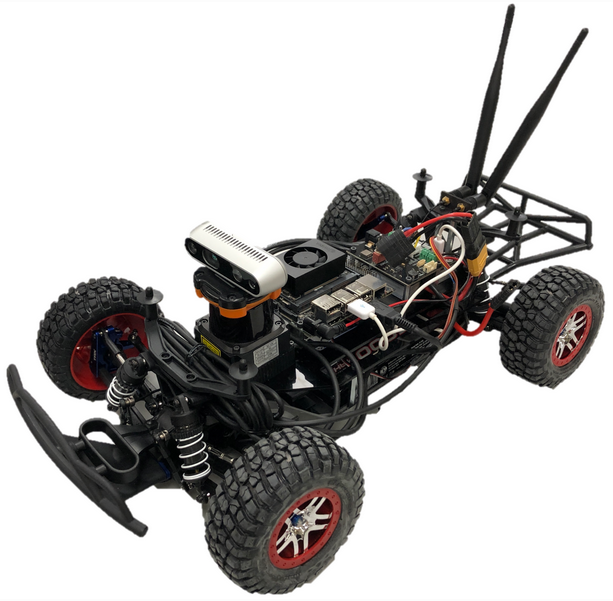
\includegraphics[width=.4\textwidth]{contents/chapt1/figs/f1tenth_car.png}
  \captionof{figure}[The F1tenth standard racecar]{The F1tenth standard vehicle, built on the chassis of a miniature RC car \cite{f1tenth}.}
  \label{fig:f1tenth_car}
\end{figure}

\section{Research motivation}

Racing vehicles such as F1tenth cars are equipped with light detection and ranging (LiDAR) scanners, inertial measurement units (IMU) and rotational encoders.
As with algorithms intended to be applied to the road-going case, autonomous racing algorithms must convert data from these sensors into steering and throttle actuator commands.
Furthermore, racing algorithms should run on-board the vehicle hardware \cite{Babu2020, f1tenth} to effectively scale when considering scenarios where many vehicles are present, such as on public roads.

The goal of racing is to output actuator commands that safely move a vehicle around a track in the shortest possible time.
Therefore, autonomous racing algorithms most optimise for two objectives;
these are (a) performance, i.e., operating the vehicle at the handling limits to achieve the fastest lap time, and (b) safety, which is to ensure that the vehicle does not collide with the track boundary or obstacles such as other cars.
These two objectives are inherently in conflict with each other because operating the vehicle close to its handling limit increases the risk of losing control \cite{Betz2021}.


Another key challenge in developing autonomous racing algorithms is robustness towards real-world transfer.
Most algorithms undergo development in simulation before their deployment on physical vehicles \cite{Babu2020, Zhou2020}.
To ensure a consistent environment between training and deployment, simulators attempt to replicate the real world as closely as possible.
This involves employing system identification techniques to create precise vehicle dynamics models \cite{Zhou2020}.

Estimating the parameters of the vehicle model poses challenges due to the dynamic nature of the driving task. 
In fact, it is inevitable that these parameters undergo changes over time \cite{Zhao2017}.
As a result, it is likely that the vehicle dynamics model employed during training does not align with the real-world vehicle dynamics. 
This phenomenon, known as model mismatch, leads to a decline in performance \cite{Ghignone2022}. 
Since some level of model mismatch is always present, accurate system identification alone is insufficient to ensure the vehicle's safety. 
It is imperative that autonomous vehicles exhibit robustness towards modeling errors.
% This thesis aims to improve the performance of learning-based algorithms where practical model mismatches are present.

% \section{Research motivation}

A recent breakthrough in autonomous racing was the introduction of learning-based solutions for vehicle control.
Learning-based solutions are commonly implemented within an end-to-end algorithm architecture, whereby a deep neural network (DNN) is trained to map sensor data directly to actuator commands \cite{Betz2021}.
End-to-end approaches have achieved excellent results in scenarios that are considered extremely challenging for previous classical approaches that separate the planning and control tasks, and rely on optimisation algorithms to perform planning.
These scenarios include racing with low computational budgets \cite{Evans2021a, Tatulea-Codrean2020} and racing against multiple vehicles \cite{Song2021, Wurman2022}.
However, learning-based approaches for vehicle control lag behind classical approaches in terms of their robustness towards model mismatch \cite{Chisari2021}.

Research efforts into addressing this challenge in learning-based approaches have largely been limited to modifying the neural network training process.
For example, \emph{sim-to-real} best practices include randomising vehicle model parameters during training \cite{Ivanov2020}, or retraining the DNN after deployment \cite{Zhou2020}.
Despite these efforts, the performance of learning-based methods are still negatively affected and have the tendency to crash when there is model mismatch present \cite{hsu2022}.



% This thesis aims to improve the performance of learning-based algorithms where practical model mismatches are present.

% A large part of the difficulty is that DRL techniques rely on an assumed vehicle dynamics model to train the neural network.
% However, this vehicle model is only an approximation of the real system dynamics. 
% Discrepancies always exist between the simulated and actual vehicle dynamics due to the difficulty of measuring the model parameters \cite{Hewing2018}. 
% These model inaccuracies cause a degradation in algorithm performance during physical deployment that can have catastrophic consequences.
% This is known as the \emph{sim2real} gap \cite{Ivanov2020}.

% % Research efforts into addressing the sim2real gap in learning-based approaches have largely been limited to modifying the training process to account for vehicle model uncertainty.
% % For example, sim2real best practices include randomising vehicle model parameters during training, or retraining the neural network after deployment \cite{Zhou2020}.

% A promising method to address the sim2real issues of current learning-based solutions is to include ideas from classical approaches. 
% Classical architectures decouple the driving task into a series of modules with specific functions.
% The task of planning a desired path and velocity profile (i.e., trajectory planning), and ensuring that the vehicle follows that trajectory (i.e., control) are handled separately. 
% Well designed control algorithms allow classical approaches to overcome the sim2real gap by minimising the the error between the actual and planned trajectory \cite{Betz2021}. 

% Approaches that synthesise classical and end-to-end architectures are known as partial end-to-end.
% These approaches utilise the modularised structure of the classical architecture, but combine or replace modules with a neural network \cite{Weiss2020}.
% Thus, partial end-to-end approaches leverage the reliability provided by the structure of classic approaches while benefitting from the heuristic nature of learning algorithms.
% However, there are relatively few research efforts related to this architecture.
% Furthermore, the use of this architecture to address the sim2real gap remains unexplored.


\section{Aims and objectives}\label{sec:objectives}

The aim of this project is to develop a learning-based autonomous racing algorithm that is robust to the vehicle modelling errors associated with real-world deployment.
As such, our racing algorithm must minimise lap time and drive safely under model mismatch conditions.
The racing scenario that we consider is a single-vehicle time trial, whereby the vehicle must complete a single lap while being alone on the track.
Furthermore, our proposed solution should be compared to previous learning-based methods for autonomous racing.
Therefore, our research is split into the following tasks:
\begin{enumerate}
    \item Investigate the literature regarding methods for developing autonomous racing algorithms, with focus on methods that are robust to vehicle modelling error.
    % \item Derive a suitable vehicle dynamics model that captures dynamics close to the edge of the handling limit.
    \item Identify and implement an appropriate simulation that captures vehicle dynamics close to the edge of the handling limit.
    \item Identify and implement an appropriate baseline learning-based autonomous racing algorithm.
    \item Design a learning based autonomous racing algorithm that is robust to vehicle modelling errors.
    \item Simulate the baseline and proposed racing algorithms under practical model mismatch conditions.
\end{enumerate}


\section{Solution overview}\label{sec:Solution_overview}



\section{Document outline}
\label{sec:outline}

Chapter \ref{chp:litreview} constitutes an overview of the existing approaches to solving the autonomous racing problem in literature, with a focus on methods for developing algorithms that are robust to vehicle modelling errors. Both classical and learning-based solutions are discussed.
We follow our literature study with the necessary theoretical background to understand the learning-based approaches used in this project in Chapters \ref{chp:anns} and \ref{chp:rl}.
Chapter \ref{chp:modelling} then describes our vehicle model and simulation setup.

We identify and describe an appropriate learning-based baseline algorithm in Chapter \ref{chp:end_to_end_autonomous_racing}.
Our racing algorithm that is robust to vehicle modelling error is described in Chapter \ref{chp:partial_end_to_end_autonomous_racing}.
The experiments that were performed under model mismatch conditions are found in Chapter \ref{chp:racing}.
The thesis is then concluded in Chapter \ref{chp:conclusion} with a summary of the work completed, as well as recommendations for future work.
